%% This is file `elsarticle-template-1-num.tex',
%%
%% Copyright 2009 Elsevier Ltd
%%
%% This file is part of the 'Elsarticle Bundle'.
%% ---------------------------------------------
%%
%% It may be distributed under the conditions of the LaTeX Project Public
%% License, either version 1.2 of this license or (at your option) any
%% later version.  The latest version of this license is in
%%    http://www.latex-project.org/lppl.txt
%% and version 1.2 or later is part of all distributions of LaTeX
%% version 1999/12/01 or later.
%%
%% The list of all files belonging to the 'Elsarticle Bundle' is
%% given in the file `manifest.txt'.
%%
%% Template article for Elsevier's document class `elsarticle'
%% with numbered style bibliographic references
%%
%% $Id: elsarticle-template-1-num.tex 149 2009-10-08 05:01:15Z rishi $
%% $URL: http://lenova.river-valley.com/svn/elsbst/trunk/elsarticle-template-1-num.tex $
%%
%%\documentclass[preprint, 12pt]{elsarticle}

%% Use the option review to obtain double line spacing
 \documentclass[preprint, review,12pt]{elsarticle}

%% Use the options 1p,twocolumn; 3p; 3p,twocolumn; 5p; or 5p,twocolumn
%% for a journal layout:
%% \documentclass[final,1p,times]{elsarticle}
%% \documentclass[final,1p,times,twocolumn]{elsarticle}
%% \documentclass[final,3p,times]{elsarticle}
%% \documentclass[final,3p,times,twocolumn]{elsarticle}
%% \documentclass[final,5p,times]{elsarticle}
%% \documentclass[final,5p,times,twocolumn]{elsarticle}

%% if you use PostScript figures in your article
%% use the graphics package for simple commands
%% \usepackage{graphics}
%% or use the graphicx package for more complicated commands
%% \usepackage{graphicx}
%% or use the epsfig package if you prefer to use the old commands
%% \usepackage{epsfig}

%% The amssymb package provides various useful mathematical symbols
\usepackage{amssymb}
%% The amsthm package provides extended theorem environments
%% \usepackage{amsthm}

%% The lineno packages adds line numbers. Start line numbering with
%% \begin{linenumbers}, end it with \end{linenumbers}. Or switch it on
%% for the whole article with \linenumbers after \end{frontmatter}.
\usepackage{lineno}

%% natbib.sty is loaded by default. However, natbib options can be
%% provided with \biboptions{...} command. Following options are
%% valid:

\usepackage{bm}

%Griffiths' uses this script r for the separation vector. 

\def\r{{\mbox{$\resizebox{.09in}{.08in}{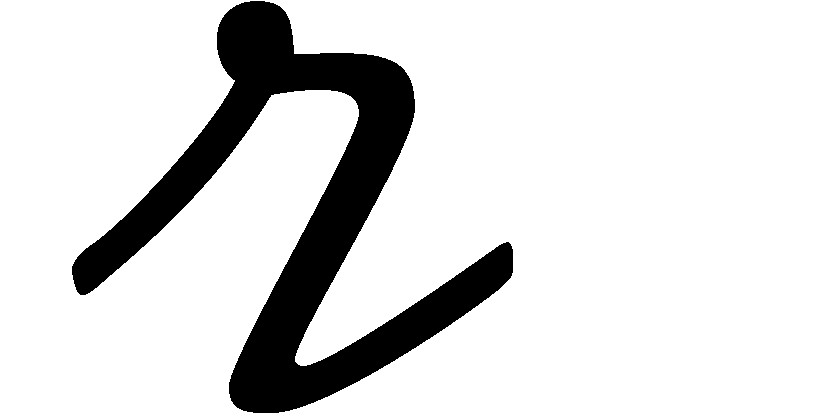
\includegraphics[trim= 1em 0 14em 0,clip]{images/ScriptR.pdf}}$}}}

\def\br{{\mbox{$\resizebox{.09in}{.08in}{
\includegraphics[trim= 1em 0 14em 0,clip]{images/BoldR.pdf}}$}}}
\def\hr{{\mbox{$\hat \br$}}}

%For use in electrodynamics instead of having to write out these prefactors every time

\def\k{\frac{1}{4 \pi \epsilon_0}}
\def\m{\frac{\mu_0}{4\pi}}
\def\x{\times}
\def\.{\cdot}
\def\b{\textbf}
\def\bell{\bm{\ell}}

%%   round  -  round parentheses are used (default)
%%   square -  square brackets are used   [option]
%%   curly  -  curly braces are used      {option}
%%   angle  -  angle brackets are used    <option>
%%   semicolon  -  multiple citations separated by semi-colon
%%   colon  - same as semicolon, an earlier confusion
%%   comma  -  separated by comma
%%   numbers-  selects numerical citations
%%   super  -  numerical citations as superscripts
%%   sort   -  sorts multiple citations according to order in ref. list
%%   sort&compress   -  like sort, but also compresses numerical citations
%%   compress - compresses without sorting
%%
%% \biboptions{comma,round}

% \biboptions{}


\journal{Journal Name}

\begin{document}

\begin{frontmatter}

%% Title, authors and addresses

%% use the tnoteref command within \title for footnotes;
%% use the tnotetext command for the associated footnote;
%% use the fnref command within \author or \address for footnotes;
%% use the fntext command for the associated footnote;
%% use the corref command within \author for corresponding author footnotes;
%% use the cortext command for the associated footnote;
%% use the ead command for the email address,
%% and the form \ead[url] for the home page:
%%
%% \title{Title\tnoteref{label1}}
%% \tnotetext[label1]{}
%% \author{Name\corref{cor1}\fnref{label2}}
%% \ead{email address}
%% \ead[url]{home page}
%% \fntext[label2]{}
%% \cortext[cor1]{}
%% \address{Address\fnref{label3}}
%% \fntext[label3]{}

\title{Electrodynamics}

%% use optional labels to link authors explicitly to addresses:
%% \author[label1,label2]{<author name>}
%% \address[label1]{<address>}
%% \address[label2]{<address>}

\author{Joshua}

%\address{Address}

%\begin{abstract}
%% Text of abstract
%Abstract
%\end{abstract}

\end{frontmatter}

%%
%% Start line numbering here if you want
%%
%%\linenumbers

%% main text

\tableofcontents

\section{Introduction}

I am starting with Griffith's fourth edition of introduction to electrodynamics. I also have volume 1 of the Pauli lectures which goes over electrodynamics. Finally I have Jackson which I do not think I will be using to prep for the qualifying exam. \cite{GriffithsEM} \cite{PauliEM} \cite{Jackson}

I will be skipping mathematical introductions as I will consolidate all of that into a different text at a different time. In this text's current form, I have just been going through Griffiths and copying down a lot of the equations from there. I hope to be able to go back and put more of my voice into these notes once I have finished going over Griffiths' book.

\section{Basic Electrostatics}



\subsection{Coulomb's Law}

The basic approach to electrostatics involves Coulomb's law,

\begin{equation}
    \b{F} = \k\frac{qQ}{\r^2}\hr.
\end{equation}

This approach deals with source charges, which are point like objects that carry some charge, q. $\epsilon_0$ is the permittivity of free space, equal to $8.85 \x 10^{-12} \frac{C^2}{N \. m^2}$. This equation is more or less postulating and then checked via experiment. Lets use this as one of our postulates of electrostatics. Once we move to electrodynamics this can be derived from Maxwell's equations. Because this equation is linear with respect to q or Q, then the law of superposition can be used when calculating out the total force on a particular charge.

Another fundamental equation of electrostatics is the definition of the electric field, 

\begin{equation}
    \b{F} \equiv q\b{E}.
\end{equation}

So combining what we have so far, the electric field for electrostatics is equal to,

\begin{equation}
    \b{E}(\b{r}) = \frac{1}{4 \pi \epsilon_0} \sum_{i=1}^n \frac{q_i}{\r^2} \hr
\end{equation}

This equation can be useful for a small amount of charges, or some very symmetrical cases but for a lot of what is done in electrostatics, you will be facing continuous charge distributions rather than this discrete form.


\subsection{Continuous Charge Distributions}

To deal with continuous charge distributions we have to switch out the summation for an integral and what we are left with is,

\begin{equation}
    \b{E}(\b{r}) = \k \int \frac{1}{\r^2}\hr dq.
\end{equation}

That dq though can be a tricky thing to establish. Usually instead of a dq, you would want it in terms of a distance. We can rewrite dq for the one-dimensional case to be equal to $\frac{dq}{dl} dl$. In problems $\frac{dq}{dl}$ is normally given to you as the linear charge distribution $\lambda$. Similarly for two-dimensions and three-dimensions we have $dq = \frac{dq}{da}da$ and $dq = \frac{dq}{d\tau}d\tau$ respectively. $\frac{dq}{da}$ is normally given as the surface charge density $\sigma$ and $\frac{dq}{d\tau}$ is normally given as the volume charge density $\rho$.


An example, is if you have a long wire, the electric field produced by it would be equal to,

\begin{equation}
    \b{E}(z) = \k \frac{2\lambda}{z} \hat{\b z}.
\end{equation}

The equations for a sphere and plane will be worked out by me later and added.

\subsection{Gauss's Law}

One of the staples of the theory of electrodynamics is Gauss's law which relates the Electric flux to the enclosed charge. Electric flux is defined by

\begin{equation}
    \Phi_E \equiv \int_S \b{E}\. d\b{a}.
\end{equation}

Gauss's law states that the electric flux is related to the charge enclosed by

\begin{equation}
    \oint \b{E}\. d\b{a} = \frac{Q_{enc}}{\epsilon_0}.
\end{equation}

From this integral equation we can derive a differential equation,

\begin{equation}
    \nabla \. \b{E} = \frac{\rho}{\epsilon_0},
\end{equation}

which is also called Gauss's law. 

Useful results that can be calculated from Gauss's law are uniformly charged symmetrical objects. The electric field for a uniformly charged sphere is,

\begin{equation}
    \b{E}= \frac{1}{4 \pi \epsilon_0} \frac{q}{r^2}\hat{\b r}.
\end{equation}

For a uniformly charged plane the electric field is,

\begin{equation}
    \b{E} = \frac{\sigma}{2\epsilon_0}\hat{\b n}.
\end{equation}

\subsection{Conservative Force}

Faraday's law states that for electrostatics, the electric force is conservative. In differential form this means that

\begin{equation}
    \nabla \x \b{E} = 0,
\end{equation}

and in integral form,

\begin{equation}
    \oint \b{E} \. d\b{l} = 0.
\end{equation}

I would like to note that this does not hold for electrodynamics though which will be covered later. Because the electric field is a conservative force we can define a potential to be,

\begin{equation}
    \b{E} \equiv -\nabla \phi,
\end{equation}

where $\phi$ is the electric potential or scalar potential. This potential is sometimes denoted by V instead of $\phi$ such as in Griffith's textbook.

The integral form of this is

\begin{equation}
    \phi(\b{r}) = - \int_O^r \b{E}\. d \bell.
\end{equation}

Where O is some reference point. O is normally where one defines the zero of the potential and is frequently at infinity. A case where this does not apply is the uniform plane where the electric field is not zero at infinity. 

\subsection{Laplace and Poisson Equations}

To try and simplify some problems, we will want to work with the potential rather than the electric field. To do so we need to convert Faraday's law and Gauss's law to be with respect to the electric potential. Taking Gauss's law and putting it in terms of the potential results in

\begin{equation}
    \nabla^2 \phi = -\frac{\rho}{\epsilon_0}.
\end{equation}

This is known as Poisson's equation, and when there exists no source charges then $\rho = 0$ and we get Laplace's equation,

\begin{equation}
    \nabla^2 \phi = 0.
\end{equation}

But what happens if we plug the potential into Faraday's law. What results is essentially a tautology because the curl of a gradient is zero. Therefore we only need a single equation to determine all of the physics rather than two.

Since the potential is useful quantity, we should have equations that allow us to solve for it that do not depend on the electric field. Taking the equation for a continuous charge distribution in three dimensions and substituting in the definition of the potential results in

\begin{equation}
    \phi(\b{r}) = \k \int \frac{\rho(\b{r'})}{\r}d\tau'.
\end{equation}

Sometimes it is quicker to derive the potential using this equation and then the field from that rather than jumping to the field directly. 

\subsection{Boundary Conditions}

Electric fields always have a jump discontinuity at surface charges. How much the electric field changes depends on what component you are looking at. For the perpendicular component

\begin{equation}
    E_{above}^\bot - E_{below}^\bot = \frac{\sigma}{\epsilon_0},
\end{equation}

and for the parallel component,

\begin{equation}
    E_{above}^\parallel = E_{below}^\parallel.
\end{equation}

The potential on the other hand does not have jump discontinuities because if it did then the electric field would be infinite at that point. Instead we can use our definition of the potential and put it into the equation that has the discontinuity to get back

\begin{equation}
    \frac{\partial \phi_{above}}{\partial n} - \frac{\partial \phi_{below}}{\partial n} = -\frac{\sigma}{\epsilon_0}.
\end{equation}

I have used the notation of a normal derivative without explaining it yet. The $\frac{\partial \phi}{\partial n}$ is a normal derivative and is defined as such

\begin{equation}
    \frac{\partial \phi}{\partial n} = \nabla \phi \. \hat{\b n},
\end{equation}

where $\hat{n}$ is the normal to the boundary. 


\subsection{Work and Energy}

The work it takes to move a charge from point a to point b is given by can be derived from the definition of work which is,

\begin{equation}
    W \equiv \int_a^b \b{F}\. d\bell.
\end{equation}

Taking it from there and substituting the previous discussions ideas results in

\begin{equation}
    W = q[\phi(\b{b})-\phi(\b{a})]
\end{equation}

Now let b be an arbitrary vector $\b{r}$ and let a be the reference point for where the potential is equal to zero. Then the work function takes on a different meaning and is just the potential energy of the system. Algebraically this means,

\begin{equation}
    U = q\phi(\b{r}),
\end{equation}

where U is the potential energy of the system of this single particle.

For a collection of particles the the potential energy is

\begin{equation}
    U = \frac{1}{2}\sum_{i=1}^n q_i \phi(\b{r}_i).
\end{equation}

The half comes from the fact that the sum double counts every interaction.

But so far all of this has been for discrete systems. What if we are dealing with the much more realistic continuous systems? Well through some mathematical manipulation the equation becomes 

\begin{equation}
    U = \frac{\epsilon_0}{2}\int E^2 d\tau, 
\end{equation}

where the bounds of integration are all of space.

\subsection{Conductors}

In insulators electrons must stay with their respective atoms while in conductors the electrons are free to move about. Dielectric is just another name for an insulator. Most everyday materials are either conductors or insulators. 

Some of the useful properties of a conductor are that the electric field inside a conductor is zero. This means that the charge density is also zero and the potential is some constant. More useful properties are that all the charge resides on the surface and the surface is equipotential. Lastly because of the boundary conditions, the electric field just outside a conductor must be perpendicular to the conductor's surface. 

An example of applying these principles would be for a neutral conductor that has a cavity in the middle of it. Then since it is neutral, any charge that's in the cavity must have an equal and opposite charge on the outside shell of the conductor due to Gauss's law. From this you could calculate the electric field outside the conductor, or even within the cavity.

Surface charges on a conductor will experience a force equal to 

\begin{equation}
    \b{f} = \frac{\sigma^2}{2 \epsilon_0} \hat{\b n}.
\end{equation}

Therefore there is an outward electrostatic pressure on the pressure equal to

\begin{equation}
    P = \frac{\epsilon_0}{2}E^2
\end{equation}

\subsection{Capacitors}

Capacitance is defined to be

\begin{equation}
    C \equiv \frac{Q}{\phi},
\end{equation}

and is measured in farads. This quantity is a purely geometrical one. For a parallel-plate capacitor, each of area A and distance d apart, the voltage

\begin{equation}
    \phi = \frac{Q}{A\epsilon_0}d,
\end{equation}

and thus the capacitance is,

\begin{equation}
    C = \frac{A\epsilon_0}{d}.
\end{equation}

What is the capacitance for two concentric spherical metal shells, with radii a and b is another example that is somewhat frequent. For this it can be found that

\begin{equation}
    C = 4\pi \epsilon_0 \frac{ab}{b-a}.
\end{equation}

Another thing important for capacitors is the energy stored in one. The work to charge up a capacitor is

\begin{equation}
    W = \frac{1}{2}C \phi^2
\end{equation}


\section{Potentials}

\subsection{Laplace's Equation}

Solutions to the Laplace equation come in the form of harmonic functions. For one dimension the general solution is simply

\begin{equation}
    \phi(x) = mx + b
\end{equation}

Properties of the one dimensional case that generalize to the two and three dimensional case are,

\begin{equation}
    \phi(x) = \frac{1}{2}[\phi(x+a) + \phi(x-a)],
\end{equation}

and the solutions have no local maxima or minima; the extrema occur at the end points. 

Earnshaw's Theorem states that a charged particles cannot be held in a stable equilibrium by electrostatic forces alone.

\subsection{Boundary Conditions}

You need boundary conditions to fully specify the solution to Laplace's equation. First uniqueness theorem states that the solution to Laplace's equation in some volume V is uniquely determined if $\phi$ is specified on the boundary surface S. Therefore the potential in a volume V is uniquely determined if the charge density throughout the region and the value of $\phi$ on all boundaries is specified. The second uniqueness theorem states that in a volume V surrounded by conductors and containing a specified charge density $\rho$, the electric field is uniquely determined if the total charge on each conductor is given.

\subsection{Method of Images}

Because of the uniqueness theorems we can devise a clever way to solve some problems that have a symmetry about them. If we are given some boundary conditions for $\phi$, usually involving some long grounded planes. By putting opposite charged charges in the correct locations, you can get the same boundary value problem. From the uniqueness theorem, the solutions to the two different problems must be the same. Therefore you just solve the simpler case with Coulomb's law and call it groovy.

For the example of a single charge +q that is located a distance d above an infinite grounded plane, 

\begin{equation}
    \phi(x,y,z) = \frac{1}{4 \pi \epsilon_0}(\frac{q}{\sqrt{x^2+y^2+(z-d)^2}} + \frac{-q}{\sqrt{x^2+y^2+(z+d)^2}})
\end{equation}

From here you can derive the induced charge distribution $\sigma$, which comes out to be

\begin{equation}
    \sigma(x,y) = \frac{-qd}{2\pi (x^2+y^2+d^2)^{\frac{3}{2}}}
\end{equation}

and thus the total induced charge must be -q. Note that the force can also be calculated from the method of images BUT you can not use the method of images to calculate the energy of the problem. For this problem the energy stored would only be half of the image problem,

\begin{equation}
    U = -\k\frac{q^2}{4d}
\end{equation}

\subsection{Multipole Expansion}

What is the potential for some $\rho \neq 0$ but $Q_{enc} = 0$? Well For cases of multipoles, and for the time being, dipoles, we can calculate it using the multipole expansion. To lay out the problem, what is the potential far away from two equal and opposite charges which are separated at a distance d from each other?

To start out with you would take the explicit formula for the potential would be 

\begin{equation}
    \phi(\b{r}) = \frac{1}{4\pi \epsilon_0}(\frac{q}{r_+}+\frac{-q}{r_-}).
\end{equation}

The next step is to expand out the $r_\pm$.

\begin{equation}
    r_\pm = r^2 + (d/2)^2 \mp rd\cos\theta.
\end{equation}

By using Taylor expansions and other basic approximation techniques you should end up at

\begin{equation}
    \phi(\b{r}) \cong \k \frac{qd\cos\theta}{r^2}
\end{equation}

A trick to see if your calculation is trick to see if your solution is correct, the potential should fall of like $\frac{1}{r^{n+1}}$ where n is the power of your pole. So for a hexadecapole, which is $2^4$ pole, then should fall off like $\frac{1}{r^5}$.

The general equation for the multipole expansion is

\begin{equation}
    \phi(\b{r}) = \frac{1}{4\pi \epsilon_0} \sum_{n=0}^\infty \frac{1}{r^{n+1}} \int (r')^n P_n(\cos \alpha ) \rho(\b{r}')d\tau'.
\end{equation}


Explicitly writing out the monopole and dipole terms,

\begin{equation}
    \phi_{mon}(\b{r}) = \k \frac{Q}{r},
\end{equation}

and,

\begin{equation}
    \phi_{dip}(\b{r}) = \frac{1}{4 \pi \epsilon_0}\frac{1}{r^2}\hat{r}\. \int \b{r'}\rho(\b{r'})d\tau'.
\end{equation}

In the dipole term, the integral is called the dipole moment, and is defined as

\begin{equation}
    \b{p} \equiv \int\b{r'} \rho(\b{r'})d\tau'.
\end{equation}

Using this definition we can rewrite the dipole's contribution as

\begin{equation}
    \phi_{dip}(\b{r}) = \k\frac{\b{p}\. \hat{\b r}}{r^2}.
\end{equation}

Note that for physical dipoles, $\b{p} = q\b{d}$ where $\b{d}$ is the separation vector between the positive and negative points.

\section{Electric Fields in Matter}

\subsection{Dipoles}

When a neutral object such as an atom in placed into an electric field, the electrons are pushed in one direction while the nucleus is pulled in the opposite. Even though the overall charge is neutral, the atom now becomes a dipole. This is what we mean when we say an electric field induces a dipole. When this happens we say the atom is polarized. If the field is not too strong the dipole moment is proportional to the field,

\begin{equation}
    \b{p} = \alpha \b{E}.
\end{equation}

The proportionality constant $\alpha$ is called the atomic polarizability, which is a measured quantity. For a more general case, $\alpha$ is not a scalar but actually a tensor called the polarizability tensor.  


What about for polar molecules? Well if a molecule already has some polarization $\b{p}$ then it will experience a torque when placed inside the external electric field. This torque is equal to 

\begin{equation}
    \b{N} = \b{p} \x \b{E}.
\end{equation}

This torque forces $\b{p}$ to be in the same direction as $\b{E}$. If the field is not uniform there exists a net force on the object equal to 

\begin{equation}
    \b{F} = (\b{p} \. \nabla)\b{E}.
\end{equation}

The energy of an ideal dipole in an external electric field is

\begin{equation}
    U = - \b{p} \. \b{E}.
\end{equation}

\subsection{Polarization}

So if you put a dielectric material in an electric field, what will happen is that each molecule in the material will become polarized with a polarization $\b{p}$. When examining the bulk material it is easier to look at the dipole moment per unit volume, $\b{P}$, or polarization.

To answer the question of what type of field this produces, we need to define a surface charge density and a volume charge density. Let the surface charge density be defined as 

\begin{equation}
    \sigma_b \equiv \b{P} \. \hat{\b n},
\end{equation}

and the volume charge density defined as,

\begin{equation}
    \rho_b \equiv - \nabla \. \b{P}.
\end{equation}

Using these definitions, and the formula for the potential defined earlier, you can derive

\begin{equation}
    \phi(\b{r}) = \k\oint_S \frac{\sigma_b}{\r}da' + \k \int_v \frac{\rho_b}{\r}d\tau'.
\end{equation}

So to calculate the potential, and thus the electric field, all one needs to do is examine what happens to the bound charges. What is a bound charge though? Is it math or a physical reality. Well as Griffiths puts it, "there is nothing further from the truth" than viewing these bound charges as mathematical constructs. It is called bound charges because they can not be removed from their source unlike a metal. They are a bulk feature, of many dipoles cancelling each other out and just looking at what the overall effect is. 

\subsection{Electric Displacement}

So now we want to examine how the field due to bound charges interacts with everything else. We shall attribute the name free charge, or $\rho_f$ so the "everything else." From how we defined free charge we can use that definition to say

\begin{equation}
    \rho = \rho_b + \rho_f.
\end{equation}

Now incorporating this definition into Gauss's law leads to

\begin{equation}
    \epsilon_0 \nabla \. \b{E} = - \nabla \. \b{P} + \rho_f
\end{equation}

Defining a new variable, the electric displacement,

\begin{equation}
    \b{D} \equiv \epsilon_0 \b{E} + \b{P},
\end{equation}

then allows us to rearrange the equation to be,

\begin{equation}
    \nabla \. \b{D} = \rho_f.
\end{equation}

The integral form of this is

\begin{equation}
    \oint \b{D} \. d\b{a}= Q_{f_{enc}}
\end{equation}

Boundary conditions for the electric displace are as follows,

\begin{equation}
    D_{above}^\bot - D_{below}^\bot = \sigma_f
\end{equation}

\begin{equation}
    \b{D}_{above}^\parallel - \b{D}_{below}^\parallel = \b{P}_{above}^\parallel - \b{P}_{below}^\parallel.
\end{equation}

\subsection{Dielectrics}

Just like in the atomic case, when an electric field, which is not too strong, is applied to some materials, then the polarization is proportional to the field,

\begin{equation}
    \b{P} = \epsilon_0 \chi_e \b{E}.
\end{equation}

The new proportionality constant $\chi_e$ is called the electric susceptibility, and if a material obeys this equation it is called a linear dielectric. If we were to convert the equation for electric displacement with this equation, then we would derive 

\begin{equation}
    \b{D} = \epsilon_0 (1+\chi_e)\b{E} = \epsilon \b{E}.
\end{equation}

This new constant of proportionality, $\epsilon$, is called the permittivity of the material. From this we can define can also define a new variable, the relative permittivity ( or dielectric constant ), 

\begin{equation}
    \epsilon_r \equiv 1 + \chi_e = \frac{\epsilon}{\epsilon_0}
\end{equation}

If the space is entirely filled with a homogeneous linear dielectric then this simplifies a lot of our problems because now electric displacement would be irrotational. In general though, dielectrics are not isotropic. In the general case, $\chi_e$ is actually a tensor called the susceptibility tensor. 

For homogeneous linear isotropic materials, the bound charge density can be related to the free charge density by

\begin{equation}
    \rho_b = - \frac{\chi_e}{1+\chi_e}\rho_f
\end{equation}

To compute the energy in a dielectric system, applying the definitions applied above, simplifies the equation down to

\begin{equation}
    U = \frac{1}{2}\int \b{D}\. \b{E}d\tau.
\end{equation}

This equation ONLY works for linear homogeneous isotropic dielectrics though.

For the special case of a finite parallel plate capacitor, with separation d, and width $w$, the force felt on the dielectric by the fringing fields is equal to 

\begin{equation}
    F = -\frac{\epsilon_0\chi_ew}{2d}\phi
\end{equation}

\section{Magnetostatics}

\subsection{Lorentz Law}

For electrostatics we required stationary charges, and for magnetostatics we will require steady currents.. The fundamental force law of magnetostatics is called the Lorentz force law. This law was experimentally found so I will write it as a definition,

\begin{equation}
    \b{F}_{mag} \equiv q(\b{v} \x \b{B}).
\end{equation}

Combining this with the definition of the electric field results in the full electrodynamics force equation,

\begin{equation}
    \b{F} = q(\b{E} + \b{v} \x \b{B}).
\end{equation}

The v in this equation is the velocity of the particle moving. I guess I should say now that the "magnetic forces do no work" just to go ahead and get that out of the way. Since they do no work, the motion of a particle under just a magnetic force is a circle. Thus using equation the magnetic force to the centripetal force you can get the cyclotron formula,

\begin{equation}
    B = \frac{mv}{qR}.
\end{equation}

The cyclotron frequency is thus

\begin{equation}
    \omega = \frac{QB}{m}.
\end{equation}

Another way of rewriting the Lorentz law in terms of current

\begin{equation}
    \b{F}_{mag} = I \bell \x \b{B}.
\end{equation}

Instead of just talking about one dimensional currents, there are two dimensional surface currents, and three dimensional volume currents. For two dimensional currents we define them as

\begin{equation}
    \b{K} \equiv \frac{d\b{I}}{d\ell_\bot} = \sigma \b{v},
\end{equation}

and for three dimensional currents,

\begin{equation}
    \b{J} \equiv \frac{d\b{I}}{da_\bot} =\rho \b{v}.
\end{equation}

The continuity equation stemming from charge conservation is

\begin{equation}
    \nabla \. \b{J} = - \frac{\partial \rho}{\partial t}.
\end{equation}

\subsection{Biot-Savart Law}

The Biot-Savart law is

\begin{equation}
    \b{B}(\b{r}) = \m \int \frac{\b{I} \x \hat{\r}}{\r^2}dl' = \m I \int \frac{d\bell \x \hr}{\r^2}.
\end{equation}

Here I have introduced a new constant, $\mu_0$, which is called the permeability of free space. Unless you are trying to be more precise than $10^{-16}$, you can simply use $\mu_0 = 4\pi \x 10^{-7} \frac{H}{m}$.

An example of using this would be finding the magnetic field a distance s from a long straight wire that has a current I. The magnetic field is then,

\begin{equation}
    \b{B} = \frac{\mu_0I}{2\pi s}\hat{\bm\phi}.
\end{equation}

Another common example is to find the magnetic field a distance z above the center of a circular loop of radius R, carrying a steady current I. In this case the magnetic field is

\begin{equation}
    \b{B}(\b{z}) = \frac{\mu_0I}{2} \frac{R^2}{(R^2+z^2)^\frac{3}{2}}\hat{\b z}.
\end{equation}

\subsection{Ampere's Law}

So we have arrived at another of Maxwell's equations, Ampere's law. Maxwell will add a correction to this equation later on but in the magnetostatics case Ampere's law works just fine. Ampere's law is analogous to Gauss's law for magnetostatics. Written in integral form it is,

\begin{equation}
    \oint \b{B} \. d\b{l} = \mu_0 I_{enc},
\end{equation}

while written in differential form is,

\begin{equation}
    \nabla \x \b{B} = \mu_0 \b{J}.
\end{equation}

Like Gaussian surfaces, these one dimensional loops are called Amperian loops. This is one of the staples of magnetostatics to be able to calculate the magnetic field due to some current. 

Now the divergence of the magnetic field is fairly simple, simpler in fact than the electrostatics case. This is also one of Maxwell's equations, and is

\begin{equation}
    \nabla \. \b{B} = 0.
\end{equation}

All this is saying is that in nature, there does not exist magnetic point charges, i.e. magnetic monopoles. 

\subsection{Magnetic Vector Potential}

For electrostatics we took advantage of the fact that $\nabla \x \b{E} = 0$ to define a scalar potential. Now for magnetostatics we will take advantage of $\nabla \. \b{B} = 0$ to define a vector potential. vector calculus identities allow us to define a vector such that,

\begin{equation}
    \b{B} = \nabla \x \b{A}.
\end{equation}

One of the features of this vector potential is that we can define it in such a way that it is divergenceless. Now this is picking a particular gauge is called the Coulomb gauge, or radiation gauge. What is this gauge I'm referencing? Well a gauge is just a systematic way to set a fixed point in a potential, usually the zero. There are other gauges, such as the Lorenz gauge which can be useful for relativistic problems that we will explore later. Converting some of the previous equations into forms dependent on the vector potential we get,

\begin{equation}
    \nabla^2 \b{A} = - \mu_0 \b{J},
\end{equation}

and,

\begin{equation}
    \b{A}(\b{r)} = \m \int \frac{\b{J(\b{r'})}}{\r}d\tau'.
\end{equation}

\subsection{Boundary Conditions}

Just like for electrostatics we have some boundary conditions for the magnetic field at boundaries. Very creative wording there. Anyways, 

\begin{equation}
    B_{above}^\bot = B_{below}^\bot
\end{equation}

is the boundary condition for the perpendicular component of the magnetic field. Note that this is analogous to the boundary condition for the parallel portion of the electric field. For the parallel portion of the magnetic field,

\begin{equation}
    B_{above}^\parallel - B_{below}^\parallel = \mu_0 K.
\end{equation}

This reminds me of the perpendicular portion of the electric field! The boundary conditions for the magnetic and electric fields essentially flipped versions of each other. To combine the magnetic field boundary equations into a single vector equation

\begin{equation}
    \b{B}_{above} - \b{B}_{below}= \mu_0 (\b{K} \x \hat{\b n}).
\end{equation}

\subsection{Multipole Expansion}

Harking back to electrostatics again, the magnetic vector potential can be written in terms of a multipole expansion. To show what it looks like

\begin{equation}
    \b{A}(\b{r}) = \m I \sum_{n=0}^\infty \frac{1}{r^{n+1}}\oint (r')^n  P_n(\cos\alpha) d\bell '.
\end{equation}

Now something to note is that THERE IS NO MAGNETIC MONOPOLE as we stated earlier thus the first term always vanishes. So the first non-vanishing term is the dipole term which is

\begin{equation}
    \b{A}_{dip}(\b{r}) = \m \frac{\b{m} \x \hat{\b r}}{r^2},
\end{equation}

where $\b{m}$ is the magnetic dipole moment, which is defined to be

\begin{equation}
    \b{m} \equiv I\b{a}.
\end{equation}

$b{a}$ is the vector area of the loop, which for most simple cases is $a\hat{n}$. From this we can derive what the magnetic field due to a dipole must be

\begin{equation}
    \b{B}_{dip}(\b{r}) = \m \frac{1}{r^3}[3(\b{m} \. \hat{r})\hat{r} - \b{m}].
\end{equation}















%% The Appendices part is started with the command \appendix;
%% appendix sections are then done as normal sections
%% \appendix

%% \section{}
%% \label{}

%% References
%%
%% Following citation commands can be used in the body text:
%% Usage of \cite is as follows:
%%   \cite{key}          ==>>  [#]
%%   \cite[chap. 2]{key} ==>>  [#, chap. 2]
%%   \citet{key}         ==>>  Author [#]

%% References with bibTeX database:

\bibliographystyle{model1-num-names}
\bibliography{sample.bib}

%% Authors are advised to submit their bibtex database files. They are
%% requested to list a bibtex style file in the manuscript if they do
%% not want to use model1-num-names.bst.

%% References without bibTeX database:

%\begin{thebibliography}{00}

%% \bibitem must have the following form:
%%   \bibitem{key}...
%%

% \bibitem{}

% \end{thebibliography}

%\appendix

%Appendix

\end{document}

%%
%% End of file `elsarticle-template-1-num.tex'.
